\documentclass[12pt,a4paper]{article}

% ─── Page Layout ───────────────────────────────────────────────────────────────
\usepackage[a4paper, margin=0.8in, headheight=14pt]{geometry}

% ─── Fonts (XeLaTeX) ───────────────────────────────────────────────────────────
\usepackage{fontspec}
\usepackage{unicode-math}
\setmainfont{TeX Gyre Pagella}
\setmonofont[Scale=0.88]{TeX Gyre Cursor}
\setmathfont{Latin Modern Math}

% ─── Packages ──────────────────────────────────────────────────────────────────
\usepackage{xcolor}
\usepackage{colortbl}
\usepackage{titlesec}
\usepackage{enumitem}
\usepackage{tabularx}
\usepackage{booktabs}
\usepackage{array}
\usepackage{amsmath}
\usepackage{tikz}
\usetikzlibrary{shapes.geometric, arrows.meta, positioning, calc, fit, decorations.pathreplacing, patterns}
\usepackage{tcolorbox}
\tcbuselibrary{skins, breakable}
\usepackage{hyperref}
\usepackage{fancyhdr}
\usepackage{graphicx}
\usepackage{microtype}
\hyphenpenalty=10000
\exhyphenpenalty=10000
\sloppy
\usepackage{caption}
\usepackage{setspace}
\usepackage{multirow}
\usepackage{tocloft}

% ─── Q&A helper ────────────────────────────────────────────────────────────────
\newcommand{\Q}[1]{\textbf{#1}\par\noindent\ignorespaces}

% ─── Colour Palette ────────────────────────────────────────────────────────────
\definecolor{myred}{RGB}{196,30,58}
\definecolor{mydark}{RGB}{30,30,50}
\definecolor{mygreen}{RGB}{14,120,80}
\definecolor{myteal}{RGB}{0,130,140}
\definecolor{myamber}{RGB}{180,100,0}
\definecolor{mypurple}{RGB}{100,30,160}
\definecolor{mygray}{RGB}{246,247,249}
\definecolor{mgframe}{RGB}{180,185,200}
\definecolor{watermark}{RGB}{145,150,170}
\definecolor{hdrred}{RGB}{250,232,235}
\definecolor{hdrgreen}{RGB}{220,244,233}
\definecolor{hdrteal}{RGB}{220,242,244}
\definecolor{hdramber}{RGB}{253,242,215}
\definecolor{hdrpurple}{RGB}{238,228,255}
\definecolor{hdrgray}{RGB}{238,240,245}
\definecolor{rowalt}{RGB}{250,251,253}

% ─── Section Formatting ────────────────────────────────────────────────────────
\titleformat{\section}
  {\large\bfseries\color{myred}}{\thesection.}{0.5em}{}
  [\vspace{1pt}{\color{myred}\rule{\linewidth}{0.8pt}}]
\titleformat{\subsection}
  {\normalsize\bfseries\color{myteal}}{\thesubsection}{0.5em}{}
\titlespacing*{\section}{0pt}{18pt}{7pt}
\titlespacing*{\subsection}{0pt}{11pt}{4pt}

% ─── Paragraph ─────────────────────────────────────────────────────────────────
\setlength{\parindent}{0pt}
\setlength{\parskip}{4pt}

% ─── TOC Styling ───────────────────────────────────────────────────────────────
\renewcommand{\cfttoctitlefont}{\large\bfseries\color{myred}}
\renewcommand{\cftaftertoctitle}{\par\noindent{\color{myred}\rule{\linewidth}{0.8pt}}}
\setlength{\cftbeforetoctitleskip}{0pt}
\setlength{\cftaftertoctitleskip}{6pt}
\renewcommand{\cftsecfont}{\normalsize\bfseries\color{mydark}}
\renewcommand{\cftsecpagefont}{\normalsize\bfseries\color{mydark}}
\renewcommand{\cftsecleader}{\cftdotfill{\cftdotsep}}
\setlength{\cftbeforesecskip}{7pt}
\renewcommand{\cftsubsecfont}{\small\color{mydark}}
\renewcommand{\cftsubsecpagefont}{\small\color{mydark}}
\setlength{\cftbeforesubsecskip}{3pt}
\setlength{\cftsubsecindent}{1.4em}

% ─── Table helpers ─────────────────────────────────────────────────────────────
\renewcommand{\arraystretch}{1.45}
\setlength{\tabcolsep}{6pt}
\arrayrulecolor{mydark}
\newcolumntype{B}[1]{>{\small\bfseries\raggedright\arraybackslash}m{#1}}
\newcolumntype{Y}{>{\small\raggedright\arraybackslash}X}
\renewcommand{\tabularxcolumn}[1]{m{#1}}

% ─── Header / Footer ───────────────────────────────────────────────────────────
\pagestyle{fancy}
\fancyhf{}
\fancyhead[L]{\small\color{myred}\textbf{BS-M301}\;\color{mydark}--- Probability and Statistics}
\fancyhead[R]{\small\color{myteal}\textbf{Module 3 Notes}}
\fancyfoot[C]{\small\color{mydark}\thepage}
\fancyfoot[R]{\small\color{watermark}\textit{\copyright\ Biraj}}
\renewcommand{\headrulewidth}{0.5pt}
\renewcommand{\footrulewidth}{0.3pt}

% ─── Hyperref ──────────────────────────────────────────────────────────────────
\hypersetup{
  colorlinks=true, linkcolor=myteal, urlcolor=myteal,
  pdfauthor={Biraj Sarkar (CGEC)},
  pdftitle={BS-M301 --- Module 3 Notes: Bivariate Distributions, Sums, Quotients and Bayes Rule}
}

% ─── tcolorbox styles ──────────────────────────────────────────────────────────
\tcbset{
  tikzbox/.style={
    colback=mygray, colframe=mgframe, boxrule=0.6pt, arc=4pt,
    left=8pt, right=8pt, top=6pt, bottom=6pt,
    colbacktitle=mgframe, coltitle=mydark,
    fonttitle=\small\bfseries
  },
  defbox/.style={
    colback=hdrgreen, colframe=mygreen, boxrule=0.8pt, arc=4pt,
    left=9pt, right=9pt, top=6pt, bottom=6pt,
    colbacktitle=mygreen, coltitle=white,
    fonttitle=\small\bfseries
  },
  formulabox/.style={
    colback=hdrteal, colframe=myteal, boxrule=0.8pt, arc=4pt,
    left=9pt, right=9pt, top=7pt, bottom=7pt,
    colbacktitle=myteal, coltitle=white,
    fonttitle=\small\bfseries
  },
  examplebox/.style={
    colback=hdramber, colframe=myamber, boxrule=0.8pt, arc=4pt,
    left=9pt, right=9pt, top=6pt, bottom=6pt,
    colbacktitle=myamber, coltitle=white,
    fonttitle=\small\bfseries
  },
  masonbox/.style={
    colback=hdrpurple, colframe=mypurple, boxrule=0.8pt, arc=4pt,
    left=9pt, right=9pt, top=6pt, bottom=6pt,
    colbacktitle=mypurple, coltitle=white,
    fonttitle=\small\bfseries
  },
  exambox/.style={
    colback=hdrpurple, colframe=mypurple, boxrule=1pt, arc=5pt,
    left=10pt, right=10pt, top=8pt, bottom=8pt,
    colbacktitle=mypurple, coltitle=white,
    fonttitle=\bfseries,
    breakable, title after break={\textbf{Frequently Asked / Viva Questions (contd.)}}
  }
}
\tcbset{breakable}
\tcbset{after={\color{black}}}

% ─── TikZ styles ───────────────────────────────────────────────────────────────
\tikzset{
  arrow/.style={-Stealth, thick, color=mydark},
  redarrow/.style={-Stealth, thick, color=myred},
  line/.style={thick, color=mydark}
}

\begin{document}

% ─── Title Page ───────────────────────────────────────────────────────────────
\begin{center}
  {\LARGE\bfseries\color{myred} BS-M301 --- Probability and Statistics}\\[5pt]
  {\normalsize\color{mydark} Semester III \quad$\bullet$\quad 3L:0T:3P \quad$\bullet$\quad 3 Credits}\\[3pt]
  {\normalsize\color{myteal}\textbf{Module 3 Exam Notes: Bivariate Distributions, Sums, Quotients and Bayes' Rule}}\\[3pt]
  {\small\color{mydark} CGEC \;$|$\; B.Tech ECE (2023--27) \;$|$\; \textit{Biraj Sarkar}}
\end{center}
\vspace{2pt}
\noindent{\color{myred}\rule{\linewidth}{1.5pt}}
\vspace{2pt}

\hypersetup{linkcolor=mydark}
\tableofcontents
\hypersetup{linkcolor=myteal}
\newpage

% ───────────────────────────────────────────────────────────────────────────────
\section{Bivariate Distributions and Their Fundamental Properties}
% ───────────────────────────────────────────────────────────────────────────────

In numerous engineering problems, physical phenomena involve the simultaneous observation of two interdependent random quantities, such as the in-phase and quadrature components of an RF communication signal $(I, Q)$, transmitter voltage and received current $(V, I)$, or temperature and humidity. These are modeled jointly as a \textbf{two-dimensional (bivariate) random variable} $(X, Y): \Omega \to \mathbb{R}^2$.

\begin{tcolorbox}[defbox, title={\textbf{Definition: Joint Probability Mass and Density Functions}}]
\textbf{Discrete Bivariate Case (Joint PMF):}
Let $(X, Y)$ take values in a countable set of pairs $(x_i, y_j)$. The \textbf{Joint PMF} is:
\begin{equation}
  p_{XY}(x_i, y_j) = P(X = x_i, Y = y_j)
\end{equation}
Axioms: (1) $p_{XY}(x_i, y_j) \ge 0, \quad \forall (i, j)$, \quad (2) $\displaystyle\sum_{i} \sum_{j} p_{XY}(x_i, y_j) = 1$.

\textbf{Continuous Bivariate Case (Joint PDF):}
$(X, Y)$ is jointly continuous if there exists an integrable surface $f_{XY}: \mathbb{R}^2 \to \mathbb{R}$ such that for any two-dimensional region $D \subseteq \mathbb{R}^2$:
\begin{equation}
  P((X, Y) \in D) = \iint_D f_{XY}(x, y) \, dx dy
\end{equation}
Axioms:
\begin{align}
  \textbf{Non-negativity:} \quad & f_{XY}(x, y) \ge 0, \quad \forall (x, y) \in \mathbb{R}^2 \\[4pt]
  \textbf{Unit Volume:} \quad & \int_{-\infty}^\infty \int_{-\infty}^\infty f_{XY}(x, y) \, dx dy = 1
\end{align}
\end{tcolorbox}

\subsection{Joint Cumulative Distribution Function (Joint CDF)}
The \textbf{Joint CDF} of $(X, Y)$ is defined as the probability of the infinite quadrant to the south-west of $(x, y)$:
\begin{equation}
  F_{XY}(x, y) = P(X \le x, Y \le y) =
  \begin{cases}
    \displaystyle\sum_{x_i \le x} \sum_{y_j \le y} p_{XY}(x_i, y_j), & \text{(Discrete)} \\[10pt]
    \displaystyle\int_{-\infty}^x \int_{-\infty}^y f_{XY}(u, v) \, dv du, & \text{(Continuous)}
  \end{cases}
\end{equation}

\begin{tcolorbox}[formulabox, title={\textbf{Properties of the Joint CDF and Recovery of Joint PDF}}]
\begin{enumerate}[leftmargin=*, itemsep=3pt]
  \item \textbf{Boundary Limits:}
  \begin{align}
    F_{XY}(-\infty, y) &= 0, \qquad F_{XY}(x, -\infty) = 0, \qquad F_{XY}(-\infty, -\infty) = 0 \\[2pt]
    F_{XY}(+\infty, +\infty) &= 1
  \end{align}
  \item \textbf{Marginal Recovery from Joint CDF:}
  \begin{equation}
    F_X(x) = \lim_{y \to +\infty} F_{XY}(x, y) = F_{XY}(x, \infty), \qquad F_Y(y) = \lim_{x \to +\infty} F_{XY}(x, y) = F_{XY}(\infty, y)
  \end{equation}
  \item \textbf{Recovery of Continuous Joint PDF by Partial Differentiation:}
  At every continuity point of $f_{XY}(x, y)$:
  \begin{equation}
    f_{XY}(x, y) = \frac{\partial^2}{\partial x \partial y} F_{XY}(x, y) = \frac{\partial^2}{\partial y \partial x} F_{XY}(x, y)
  \end{equation}
  \item \textbf{Rectangle Probability Rule:} For any rectangular region $[x_1, x_2] \times [y_1, y_2]$:
  \begin{align}
    P(x_1 < X \le x_2, \; y_1 < Y \le y_2) = \; & F_{XY}(x_2, y_2) - F_{XY}(x_1, y_2) \nonumber \\[2pt]
                                                & - F_{XY}(x_2, y_1) + F_{XY}(x_1, y_1) \ge 0
  \end{align}
\end{enumerate}
\end{tcolorbox}

\subsection{Marginal Distributions}
The individual distribution of one variable obtained by integrating or summing out the other variable over its entire support is termed the \textbf{marginal distribution}.
\begin{align}
  \textbf{Marginal PMFs:} \quad & p_X(x_i) = \sum_{j} p_{XY}(x_i, y_j), \qquad p_Y(y_j) = \sum_{i} p_{XY}(x_i, y_j) \\[4pt]
  \textbf{Marginal PDFs:} \quad & f_X(x) = \int_{-\infty}^\infty f_{XY}(x, y) \, dy, \qquad f_Y(y) = \int_{-\infty}^\infty f_{XY}(x, y) \, dx
\end{align}

\begin{tcolorbox}[tikzbox, title={\textbf{TikZ Schematic: Geometric Interpretation of Marginal Integration across Joint Support}}]
\begin{center}
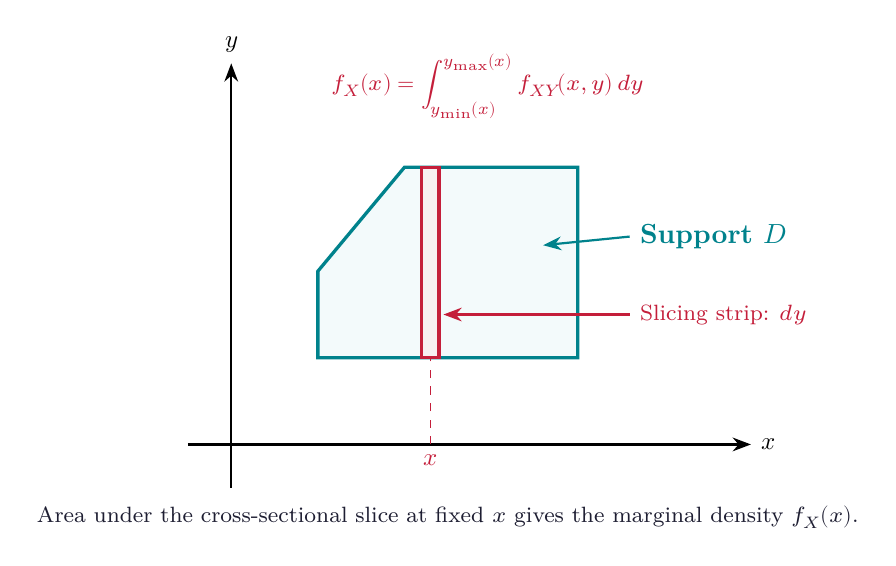
\begin{tikzpicture}[scale=1.1, every node/.style={font=\small}]
  % Axes
  \draw[-Stealth, thick] (-0.5, 0) -- (6.0, 0) node[right] {$x$};
  \draw[-Stealth, thick] (0, -0.5) -- (0, 4.4) node[above] {$y$};

  % Support region D
  \draw[very thick, color=myteal, fill=hdrteal, fill opacity=0.35]
    (1, 1) -- (4, 1) -- (4, 3.2) -- (2, 3.2) -- (1, 2) -- cycle;

  % Fixed x vertical strip
  \draw[very thick, color=myred, fill=hdrred, fill opacity=0.6] (2.2, 1) rectangle (2.4, 3.2);
  \draw[dashed, thin, color=myred] (2.3, 0) node[below] {$x$} -- (2.3, 1);

  % External Callouts on the right
  \draw[-Stealth, thick, color=myteal] (4.6, 2.4) node[right, font=\bfseries, color=myteal] {Support $D$} -- (3.6, 2.3);
  \draw[-Stealth, thick, color=myred] (4.6, 1.5) node[right, font=\footnotesize, color=myred] {Slicing strip: $dy$} -- (2.45, 1.5);

  % Annotations at top
  \node[above, color=myred, font=\footnotesize, align=center] at (3.0, 3.65) {
    $f_X(x) = \displaystyle\int_{y_{\min}(x)}^{y_{\max}(x)} f_{XY}(x, y) \, dy$
  };
  \node[below, color=mydark, font=\footnotesize] at (2.5, -0.6) {
    Area under the cross-sectional slice at fixed $x$ gives the marginal density $f_X(x)$.
  };
\end{tikzpicture}
\end{center}
\end{tcolorbox}

% ───────────────────────────────────────────────────────────────────────────────
\section{Conditional Distributions, Densities and Bayes' Rule}
% ───────────────────────────────────────────────────────────────────────────────

\begin{tcolorbox}[defbox, title={\textbf{Definition: Conditional Probability Density Function}}]
Given that the random variable $Y$ has taken on a specific numerical value $Y = y$ (where marginal density $f_Y(y) > 0$), the \textbf{conditional PDF} of $X$ given $Y = y$ is defined as:
\begin{equation}
  f_{X \mid Y}(x \mid y) = \frac{f_{XY}(x, y)}{f_Y(y)} = \frac{f_{XY}(x, y)}{\displaystyle\int_{-\infty}^\infty f_{XY}(u, y) \, du}
\end{equation}
Symmetrically, the conditional PDF of $Y$ given $X = x$ (with $f_X(x) > 0$) is:
\begin{equation}
  f_{Y \mid X}(y \mid x) = \frac{f_{XY}(x, y)}{f_X(x)} = \frac{f_{XY}(x, y)}{\displaystyle\int_{-\infty}^\infty f_{XY}(x, v) \, dv}
\end{equation}
Every conditional density satisfies the standard PDF axioms: $f_{X|Y}(x \mid y) \ge 0$ and $\int_{-\infty}^\infty f_{X|Y}(x \mid y) dx = 1$.
\end{tcolorbox}

\subsection{Conditional Expectation and the Tower Property}
\begin{itemize}[leftmargin=*, itemsep=3pt]
  \item \textbf{Conditional Expectation:} The mean of $X$ given $Y = y$ is a function of $y$:
  \begin{equation}
    E[X \mid Y = y] = \int_{-\infty}^\infty x f_{X \mid Y}(x \mid y) \, dx
  \end{equation}
  \item \textbf{Law of Iterated Expectations (Tower Property):}
  \begin{equation}
    E\left[E[X \mid Y]\right] = E[X]
  \end{equation}
  \textbf{Proof:}
  \begin{align}
    E\left[E[X \mid Y]\right] &= \int_{-\infty}^\infty \left(\int_{-\infty}^\infty x \frac{f_{XY}(x, y)}{f_Y(y)} dx\right) f_Y(y) \, dy \nonumber \\
                              &= \int_{-\infty}^\infty \int_{-\infty}^\infty x f_{XY}(x, y) \, dx dy = \int_{-\infty}^\infty x \left(\int_{-\infty}^\infty f_{XY}(x, y) dy\right) dx \nonumber \\
                              &= \int_{-\infty}^\infty x f_X(x) \, dx = E[X]
  \end{align}
  \item \textbf{Law of Total Variance (Eve's Law):}
  \begin{equation}
    \operatorname{Var}(X) = E[\operatorname{Var}(X \mid Y)] + \operatorname{Var}(E[X \mid Y])
  \end{equation}
  Total uncertainty equals the average unexplained variance plus the variance explained by $Y$.
\end{itemize}

\subsection{Bayes' Rule for Continuous and Mixed Random Variables}
\begin{tcolorbox}[formulabox, title={\textbf{Continuous and Mixed Formulations of Bayes' Rule}}]
\textbf{Continuous Inversion (Posterior Density):}
Equating $f_{XY}(x, y) = f_X(x) f_{Y|X}(y \mid x) = f_Y(y) f_{X|Y}(x \mid y)$:
\begin{equation}
  f_{X \mid Y}(x \mid y) = \frac{f_X(x) \cdot f_{Y \mid X}(y \mid x)}{f_Y(y)} = \frac{f_X(x) \cdot f_{Y \mid X}(y \mid x)}{\displaystyle\int_{-\infty}^\infty f_X(u) \cdot f_{Y \mid X}(y \mid u) \, du}
\end{equation}
where $f_X(x)$ is the \textit{prior density}, $f_{Y|X}(y \mid x)$ is the \textit{likelihood function}, and $f_{X|Y}(x \mid y)$ is the \textit{posterior density}.

\textbf{Discrete Hypothesis with Continuous Measurement (Signal Detection):}
Let $\{H_1, H_2, \dots, H_n\}$ be discrete transmitted symbols (priors $P(H_i)$) observed through continuous additive noise $Y$:
\begin{equation}
  P(H_k \mid Y = y) = \frac{P(H_k) \cdot f_{Y \mid H_k}(y)}{\displaystyle\sum_{i=1}^n P(H_i) \cdot f_{Y \mid H_i}(y)}
\end{equation}
\end{tcolorbox}

% ───────────────────────────────────────────────────────────────────────────────
\section{Bivariate Transformations and the Jacobian Method}
% ───────────────────────────────────────────────────────────────────────────────

When analyzing signal processing systems, inputs $(X, Y)$ are mapped into new output variables $(U, V)$ via mathematical functions $U = g_1(X, Y)$ and $V = g_2(X, Y)$.

\begin{tcolorbox}[defbox, title={\textbf{Theorem: Bivariate Jacobian Transformation}}]
Let $(X, Y)$ have joint PDF $f_{XY}(x, y)$ supported on set $D$. Let the transformation:
\begin{equation}
  u = g_1(x, y), \qquad v = g_2(x, y)
\end{equation}
define a one-to-one and invertible mapping from $D$ onto range $S$, with unique inverse:
\begin{equation}
  x = h_1(u, v), \qquad y = h_2(u, v)
\end{equation}
If the partial derivatives are continuous, the \textbf{Jacobian determinant} $J$ of the inverse transformation is:
\begin{equation}
  J = \frac{\partial(x, y)}{\partial(u, v)} = \det \begin{pmatrix} \dfrac{\partial x}{\partial u} & \dfrac{\partial x}{\partial v} \\[6pt] \dfrac{\partial y}{\partial u} & \dfrac{\partial y}{\partial v} \end{pmatrix} = \frac{\partial x}{\partial u}\frac{\partial y}{\partial v} - \frac{\partial x}{\partial v}\frac{\partial y}{\partial u}
\end{equation}
Then the joint PDF of $(U, V)$ over $S$ is given by:
\begin{equation}
  f_{UV}(u, v) = f_{XY}\left(h_1(u, v), h_2(u, v)\right) \cdot |J|
\end{equation}
where $|J|$ is the absolute value of the Jacobian determinant (representing the local area scaling factor: $dx dy = |J| du dv$).
\end{tcolorbox}

\begin{tcolorbox}[tikzbox, title={\textbf{TikZ Schematic: Area Element Transformation under Jacobian Mapping}}]
\begin{center}
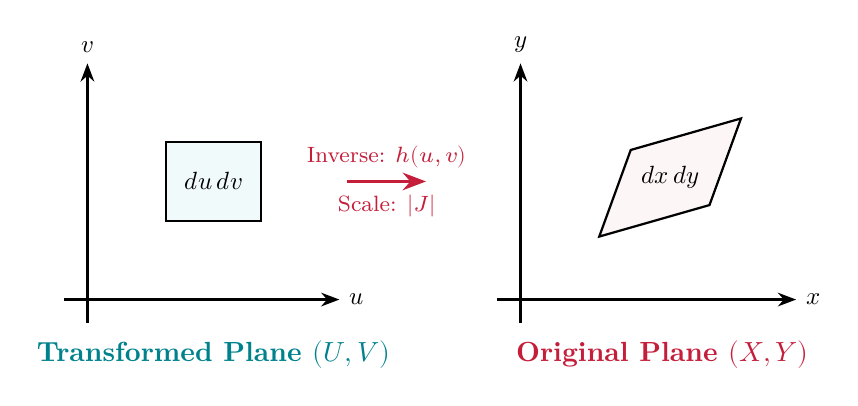
\begin{tikzpicture}[scale=1.0, every node/.style={font=\small}]
  % Left plane: (u, v)
  \begin{scope}[shift={(-3.5, 0)}]
    \draw[-Stealth, thick] (-0.3, 0) -- (3.2, 0) node[right] {$u$};
    \draw[-Stealth, thick] (0, -0.3) -- (0, 3.0) node[above] {$v$};

    \draw[thick, fill=hdrteal, fill opacity=0.4] (1, 1) rectangle (2.2, 2.0);
    \node at (1.6, 1.5) {$du \, dv$};
    \node[below, font=\bfseries, color=myteal] at (1.6, -0.4) {Transformed Plane $(U, V)$};
  \end{scope}

  % Mapping arrow
  \draw[-Stealth, very thick, color=myred] (-0.2, 1.5) -- (0.8, 1.5);
  \node[above, color=myred, font=\footnotesize] at (0.3, 1.55) {Inverse: $h(u,v)$};
  \node[below, color=myred, font=\footnotesize] at (0.3, 1.45) {Scale: $|J|$};

  % Right plane: (x, y)
  \begin{scope}[shift={(2.0, 0)}]
    \draw[-Stealth, thick] (-0.3, 0) -- (3.5, 0) node[right] {$x$};
    \draw[-Stealth, thick] (0, -0.3) -- (0, 3.0) node[above] {$y$};

    \draw[thick, fill=hdrred, fill opacity=0.4]
      (1, 0.8) -- (2.4, 1.2) -- (2.8, 2.3) -- (1.4, 1.9) -- cycle;
    \node at (1.9, 1.55) {$dx \, dy$};
    \node[below, font=\bfseries, color=myred] at (1.8, -0.4) {Original Plane $(X, Y)$};
  \end{scope}
\end{tikzpicture}
\end{center}
\end{tcolorbox}

% ───────────────────────────────────────────────────────────────────────────────
\section{Distributions of Sums and Quotients}
% ───────────────────────────────────────────────────────────────────────────────

\subsection{Distribution of the Sum $Z = X + Y$ (Convolution)}
\begin{tcolorbox}[examplebox, title={\textbf{Derivation: PDF of the Sum of Two Continuous Random Variables}}]
To find the PDF of $Z = X + Y$, introduce an auxiliary variable $W = X$.
The forward transformation is:
\begin{equation}
  z = x + y, \qquad w = x
\end{equation}
The unique inverse transformation is:
\begin{equation}
  x = w, \qquad y = z - w
\end{equation}
Computing the Jacobian determinant:
\begin{equation}
  J = \det \begin{pmatrix} \frac{\partial x}{\partial z} & \frac{\partial x}{\partial w} \\[4pt] \frac{\partial y}{\partial z} & \frac{\partial y}{\partial w} \end{pmatrix} = \det \begin{pmatrix} 0 & 1 \\ 1 & -1 \end{pmatrix} = (0)(-1) - (1)(1) = -1 \implies |J| = |-1| = 1
\end{equation}
The joint PDF of $(Z, W)$ is:
\begin{equation}
  f_{ZW}(z, w) = f_{XY}(w, z - w) \cdot |J| = f_{XY}(w, z - w)
\end{equation}
Integrating out the auxiliary variable $w$ yields the marginal PDF of the sum $Z$:
\begin{equation}
  f_Z(z) = \int_{-\infty}^\infty f_{ZW}(z, w) \, dw = \int_{-\infty}^\infty f_{XY}(w, z - w) \, dw
\end{equation}
If $X$ and $Y$ are \textbf{independent} ($f_{XY}(x, y) = f_X(x) f_Y(y)$), this becomes the fundamental \textbf{continuous convolution integral}:
\begin{equation}
  f_Z(z) = (f_X * f_Y)(z) = \int_{-\infty}^\infty f_X(w) f_Y(z - w) \, dw = \int_{-\infty}^\infty f_X(z - y) f_Y(y) \, dy
\end{equation}
\end{tcolorbox}

\subsection{Distribution of the Quotient $Z = X / Y$}
\begin{tcolorbox}[examplebox, title={\textbf{Derivation: PDF of the Quotient of Two Random Variables}}]
Let $Z = \frac{X}{Y}$. Introduce the auxiliary variable $W = Y$.
The forward transformation is:
\begin{equation}
  z = \frac{x}{y}, \qquad w = y \quad (w \ne 0)
\end{equation}
The inverse transformation is:
\begin{equation}
  x = z \cdot w, \qquad y = w
\end{equation}
The Jacobian determinant is:
\begin{equation}
  J = \det \begin{pmatrix} \frac{\partial x}{\partial z} & \frac{\partial x}{\partial w} \\[4pt] \frac{\partial y}{\partial z} & \frac{\partial y}{\partial w} \end{pmatrix} = \det \begin{pmatrix} w & z \\ 0 & 1 \end{pmatrix} = (w)(1) - (z)(0) = w \implies |J| = |w|
\end{equation}
The joint PDF of $(Z, W)$ is:
\begin{equation}
  f_{ZW}(z, w) = f_{XY}(z w, w) \cdot |w|
\end{equation}
Integrating out $w$ over $(-\infty, \infty)$ yields the general quotient density:
\begin{equation}
  f_Z(z) = \int_{-\infty}^\infty |w| f_{XY}(z w, w) \, dw
\end{equation}
If $X$ and $Y$ are independent:
\begin{equation}
  f_Z(z) = \int_{-\infty}^\infty |w| f_X(z w) f_Y(w) \, dw
\end{equation}
\end{tcolorbox}

\subsection{Quotient of Two Independent Standard Normals: The Cauchy Distribution}
\begin{tcolorbox}[examplebox, title={\textbf{Classic Result: Ratio of Independent Standard Normals follows Cauchy}}]
Let $X \sim \mathcal{N}(0, 1)$ and $Y \sim \mathcal{N}(0, 1)$ be independent. Their joint density is:
\begin{equation}
  f_{XY}(x, y) = \frac{1}{\sqrt{2\pi}} e^{-x^2/2} \cdot \frac{1}{\sqrt{2\pi}} e^{-y^2/2} = \frac{1}{2\pi} e^{-(x^2 + y^2)/2}
\end{equation}
Applying the quotient formula to $Z = X/Y$:
\begin{equation}
  f_Z(z) = \int_{-\infty}^\infty |w| \cdot \frac{1}{2\pi} e^{-(z^2 w^2 + w^2)/2} \, dw = \frac{1}{2\pi} \int_{-\infty}^\infty |w| e^{-\frac{w^2(1 + z^2)}{2}} \, dw
\end{equation}
Since the integrand is even with respect to $w$:
\begin{equation}
  f_Z(z) = \frac{2}{2\pi} \int_0^\infty w e^{-\frac{w^2(1 + z^2)}{2}} \, dw = \frac{1}{\pi} \int_0^\infty w e^{-\frac{w^2(1 + z^2)}{2}} \, dw
\end{equation}
Substitute $u = \frac{w^2(1 + z^2)}{2} \implies du = (1 + z^2) w dw \implies w dw = \frac{du}{1 + z^2}$:
\begin{equation}
  f_Z(z) = \frac{1}{\pi (1 + z^2)} \int_0^\infty e^{-u} \, du = \frac{1}{\pi (1 + z^2)} \left[-e^{-u}\right]_0^\infty = \frac{1}{\pi (1 + z^2)} (1)
\end{equation}
\begin{equation}
  f_Z(z) = \frac{1}{\pi (1 + z^2)}, \qquad -\infty < z < \infty
\end{equation}
This is the celebrated \textbf{Standard Cauchy Distribution}!
\textit{Crucial Exam Note:} For a Cauchy distribution, $\int_{-\infty}^\infty |z| \frac{1}{\pi(1+z^2)} dz = \infty$. Therefore, the Cauchy distribution has \textbf{no defined mean, no variance, and no MGF}!
\end{tcolorbox}

\begin{tcolorbox}[tikzbox, title={\textbf{TikZ Plot: Standard Cauchy PDF vs. Standard Normal Gaussian PDF}}]
\begin{center}
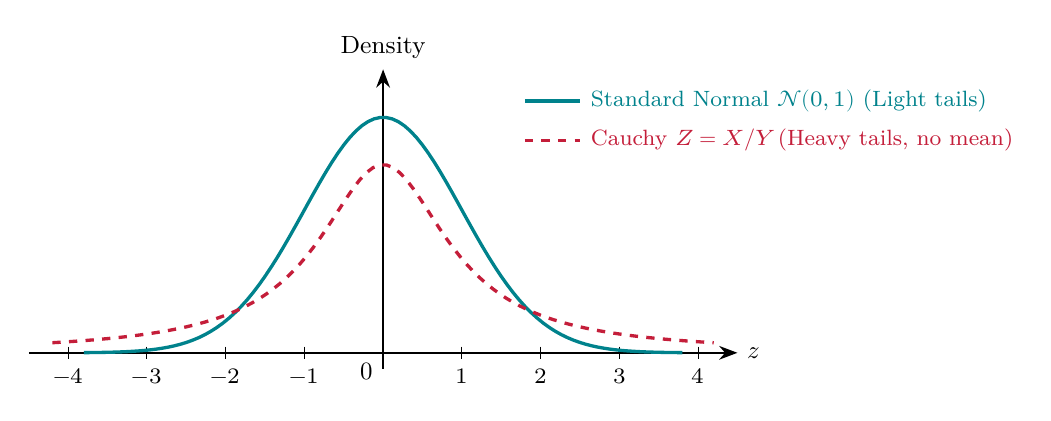
\begin{tikzpicture}[scale=1.0, every node/.style={font=\small}]
  % Axes
  \draw[-Stealth, thick] (-4.5, 0) -- (4.5, 0) node[right] {$z$};
  \draw[-Stealth, thick] (0, -0.2) -- (0, 3.6) node[above] {Density};

  % Ticks
  \foreach \x in {-4,-3,-2,-1,1,2,3,4} {
    \draw (\x, 0.08) -- (\x, -0.08) node[below] {\footnotesize $\x$};
  }
  \node[below left] at (0, 0) {$0$};

  % Standard Normal: peak 0.3989 -> scale * 7.5 = 2.99
  \draw[very thick, color=myteal, domain=-3.8:3.8, samples=100]
    plot (\x, {2.99*exp(-(\x)^2/2)});

  % Cauchy: f(z) = 1/(pi*(1+z^2)), peak at z=0 is 1/pi = 0.3183 -> scale * 7.5 = 2.39
  \draw[very thick, color=myred, dashed, domain=-4.2:4.2, samples=100]
    plot (\x, {2.39 / (1 + (\x)^2)});

  % Legend
  \draw[very thick, color=myteal] (1.8, 3.2) -- (2.5, 3.2) node[right, font=\footnotesize] {Standard Normal $\mathcal{N}(0, 1)$ (Light tails)};
  \draw[very thick, color=myred, dashed] (1.8, 2.7) -- (2.5, 2.7) node[right, font=\footnotesize] {Cauchy $Z = X/Y$ (Heavy tails, no mean)};
\end{tikzpicture}
\end{center}
\end{tcolorbox}

\newpage
% ===============================================================================
% MANDATORY QUICK REVISION PAGE
% ===============================================================================
\begin{center}
  {\large\bfseries\color{myred} Quick Revision --- Module 3}\\[1pt]
  {\small\color{mydark} Bivariate Distributions, Sums, Quotients and Bayes' Rule $|$ BS-M301}
\end{center}
\noindent{\color{myred}\rule{\linewidth}{1.0pt}}
\vspace{1pt}

\begin{tcolorbox}[formulabox, top=3pt, bottom=3pt, title={\textbf{Key Formulas and Bivariate Relations at a Glance}}]
\renewcommand{\arraystretch}{1.18}
\setlength{\tabcolsep}{4pt}
\begin{tabularx}{\linewidth}{B{3.4cm} X}
Joint PDF \& CDF & $f_{XY}(x,y) \ge 0, \; \iint f_{XY} dx dy = 1; \quad f_{XY}(x,y) = \frac{\partial^2 F_{XY}}{\partial x \partial y}$ \\[2.5pt]
Marginal Densities & $f_X(x) = \int_{-\infty}^\infty f_{XY}(x,y) dy, \quad f_Y(y) = \int_{-\infty}^\infty f_{XY}(x,y) dx$ \\[2.5pt]
Conditional Densities & $f_{X|Y}(x \mid y) = \frac{f_{XY}(x,y)}{f_Y(y)}, \quad f_{Y|X}(y \mid x) = \frac{f_{XY}(x,y)}{f_X(x)}$ \\[2.5pt]
Statistical Independence & $f_{XY}(x,y) = f_X(x) f_Y(y) \iff f_{X|Y}(x \mid y) = f_X(x)$ \\[2.5pt]
Tower Property & $E\left[E[X \mid Y]\right] = E[X], \quad \operatorname{Var}(X) = E[\operatorname{Var}(X|Y)] + \operatorname{Var}(E[X|Y])$ \\[2.5pt]
Jacobian Transform & $f_{UV}(u,v) = f_{XY}(h_1, h_2) \cdot |J|, \quad J = \det \begin{pmatrix} \frac{\partial x}{\partial u} & \frac{\partial x}{\partial v} \\ \frac{\partial y}{\partial u} & \frac{\partial y}{\partial v} \end{pmatrix}$ \\[2.5pt]
Sum \& Quotient PDFs & $Z = X+Y \implies f_Z = \int f(w, z-w) dw; \quad Z = \frac{X}{Y} \implies f_Z = \int |w| f(zw, w) dw$ \\[2.5pt]
Cauchy \& Bayes' Rule & $Z = \frac{X}{Y} \sim \text{Cauchy}: f_Z(z) = \frac{1}{\pi(1+z^2)}; \quad f_{X|Y}(x \mid y) = \frac{f_X(x) f_{Y|X}(y \mid x)}{\int_{-\infty}^\infty f_X(u) f_{Y|X}(y \mid u) du}$ \\
\end{tabularx}
\end{tcolorbox}

\vspace{1pt}

\begin{tcolorbox}[defbox, top=2pt, bottom=2pt, title={\textbf{One-Line Definitions}}]
\small
\begin{itemize}[leftmargin=12pt, itemsep=-0.6pt, topsep=0pt, parsep=0pt]
  \item \textbf{Joint PDF $f_{XY}(x,y)$:} Surface whose double integral over any region $D$ equals $P((X,Y) \in D)$.
  \item \textbf{Marginal PDF:} Individual density of one component obtained by integrating out the other variable.
  \item \textbf{Conditional PDF:} Sliced cross-sectional density of $X$ normalized by $f_Y(y)$ under $Y=y$.
  \item \textbf{Statistical Independence:} Factorization $f_{XY}(x,y) = f_X(x) f_Y(y)$ across the entire domain.
  \item \textbf{Tower Property:} Fundamental law asserting that overall expectation equals $E[E[X \mid Y]]$.
  \item \textbf{Jacobian Determinant ($J$):} Local area transformation ratio $dx dy = |J| du dv$ relating coordinate spaces.
  \item \textbf{Convolution Theorem:} Integral operation yielding the PDF of the sum of independent RVs: $f_Z = f_X * f_Y$.
  \item \textbf{Quotient Distribution:} Density $f_Z(z) = \int |w| f(zw, w) dw$ describing the ratio of two RVs.
  \item \textbf{Cauchy Distribution:} Heavy-tailed distribution $f(z) = \frac{1}{\pi(1+z^2)}$ formed by $\mathcal{N}(0,1)/\mathcal{N}(0,1)$, lacking moments.
  \item \textbf{Posterior Density:} Updated density of an unknown parameter after incorporating observation $y$.
\end{itemize}
\end{tcolorbox}

\newpage

\begin{tcolorbox}[exambox, title={\textbf{Frequently Asked / Viva Questions (Part 1)}}]
\begin{enumerate}[topsep=0pt, label=\textbf{Q\arabic*.}, itemsep=3.2pt]
  \item \Q{State the necessary and sufficient conditions for two continuous random variables $X$ and $Y$ to be independent.}
  $X$ and $Y$ are independent if and only if their joint PDF factors into the product of their marginal PDFs everywhere: $f_{XY}(x, y) = f_X(x) f_Y(y)$ for all $(x, y) \in \mathbb{R}^2$, and the support region $D$ is a product of intervals (non-coupled boundaries).

  \item \Q{How is the joint PDF obtained from the joint Cumulative Distribution Function?}
  By mixed second-order partial differentiation: $f_{XY}(x, y) = \frac{\partial^2}{\partial x \partial y} F_{XY}(x, y)$, provided the second partial derivatives exist and are continuous.

  \item \Q{State and prove the Law of Iterated Expectations (Tower Property).}
  $E\left[E[X \mid Y]\right] = E[X]$. Proof: $E[E[X \mid Y]] = \int \left(\int x \frac{f(x,y)}{f_Y(y)} dx\right) f_Y(y) dy = \iint x f(x,y) dx dy = \int x f_X(x) dx = E[X]$.

  \item \Q{What is the physical significance of the Jacobian determinant in bivariate transformations?}
  The Jacobian determinant $J = \frac{\partial(x, y)}{\partial(u, v)}$ represents the local geometric dilation factor between the original and transformed coordinate planes, ensuring conservation of probability mass: $P(dx dy) = f_{XY}(x, y) dx dy = f_{XY}(h_1, h_2) |J| du dv = f_{UV}(u, v) du dv$.

  \item \Q{Derive the PDF of the sum $Z = X + Y$ of two independent continuous random variables.}
  Let $Z = X + Y, W = X \implies X = W, Y = Z - W$. The Jacobian is $|J| = 1$. The joint density is $f_{ZW}(z, w) = f_{XY}(w, z - w) = f_X(w) f_Y(z - w)$. Integrating over $w$ gives the convolution: $f_Z(z) = \int_{-\infty}^\infty f_X(w) f_Y(z - w) dw$.

  \item \Q{Why does the absolute value $|w|$ appear in the formula for the quotient density $Z = X/Y$?}
  The Jacobian of the inverse transformation $x = z w, y = w$ is $J = \det \begin{pmatrix} w & z \\ 0 & 1 \end{pmatrix} = w$. Because an area element must always be strictly non-negative ($dx dy = |J| dz dw$), the absolute value $|J| = |w|$ must be taken.

  \item \Q{Show that the ratio of two independent standard normal random variables follows a Cauchy distribution.}
  $f_Z(z) = \frac{1}{2\pi} \int_{-\infty}^\infty |w| e^{-w^2(1+z^2)/2} dw = \frac{1}{\pi} \int_0^\infty w e^{-w^2(1+z^2)/2} dw$. Substituting $u = w^2(1+z^2)/2$ transforms the integral to $\frac{1}{\pi(1+z^2)} \int_0^\infty e^{-u} du = \frac{1}{\pi(1+z^2)}$, which is the standard Cauchy PDF.
\end{enumerate}
\end{tcolorbox}

\newpage

\begin{tcolorbox}[exambox, top=3pt, bottom=3pt, title={\textbf{Frequently Asked / Viva Questions (Part 2)}}]
\begin{enumerate}[topsep=0pt, label=\textbf{Q\arabic*.}, itemsep=1.8pt, start=8]
  \item \Q{Why does the Cauchy distribution have no mathematical expectation or variance?}
  $E[|Z|] = \frac{1}{\pi} \int_{-\infty}^\infty \frac{|z|}{1+z^2} dz = \frac{2}{\pi} \int_0^\infty \frac{z}{1+z^2} dz = \frac{1}{\pi} \left[\ln(1+z^2)\right]_0^\infty = \infty$. Because the absolute integral diverges logarithmically due to heavy polynomial tails ($\sim 1/z^2$), the mean is mathematically undefined, and all higher moments diverge.

  \item \Q{State the Law of Total Variance (Eve's Law) and interpret its terms.}
  $\operatorname{Var}(X) = E[\operatorname{Var}(X \mid Y)] + \operatorname{Var}(E[X \mid Y])$. The first term represents the average unexplained variation remaining in $X$ after conditioning on $Y$; the second term represents the variation in the conditional predictor $E[X \mid Y]$ explained by $Y$.

  \item \Q{State Continuous Bayes' Theorem and explain its role in signal estimation.}
  $f_{X|Y}(x \mid y) = \frac{f_X(x) f_{Y|X}(y \mid x)}{\int f_X(u) f_{Y|X}(y \mid u) du}$. In communications, $X$ is the transmitted signal (prior), $f_{Y|X}(y \mid x)$ is the channel noise model (likelihood), and $f_{X|Y}(x \mid y)$ is the posterior distribution used by the receiver to make Maximum A Posteriori (MAP) symbol decisions.
\end{enumerate}
\end{tcolorbox}

\vspace{2pt}

\begin{tcolorbox}[tikzbox, top=3pt, bottom=3pt, title={\textbf{Summary Matrix: Comprehensive Comparison of Bivariate Operations}}]
\par\vspace{1pt}\noindent
\begingroup
\setlength{\tabcolsep}{3.5pt}
\setlength{\extrarowheight}{1.0pt}
\renewcommand{\arraystretch}{1.15}
\begin{tabularx}{\linewidth}{|>{\small\bfseries\raggedright\arraybackslash}m{2.3cm}|>{\small\raggedright\arraybackslash}m{4.6cm}|>{\small\raggedright\arraybackslash}m{3.9cm}|Y|}
\hline
\textbf{Operation / Concept} & \textbf{Mathematical Governing Expression} & \textbf{Independence Simplification} & \textbf{Physical Meaning / Role} \\
\hline
Marginal Density & $f_X(x) = \int_{-\infty}^\infty f_{XY}(x, y) \, dy$ & $f_X(x) \int f_Y(y) dy = f_X(x)$ & Complete projection onto $X$-axis. \\
\hline
Conditional Density & $f_{X|Y}(x \mid y) = \frac{f_{XY}(x, y)}{f_Y(y)}$ & $f_{X|Y}(x \mid y) = f_X(x)$ & Updated density given knowledge $Y=y$. \\
\hline
Sum of RVs & $Z = X + Y \implies f_Z(z) = \int f_{XY}(w, z-w) dw$ & Convolution: $f_Z = f_X * f_Y$ & Total noise from independent sources. \\
\hline
Quotient of RVs & $Z = X / Y \implies f_Z(z) = \int |w| f_{XY}(zw, w) dw$ & $\int |w| f_X(zw) f_Y(w) dw$ & Signal-to-noise ratio; slope of vector. \\
\hline
Cauchy Ratio & $Z = X/Y$ for $X,Y \sim \mathcal{N}(0, 1) \implies \frac{1}{\pi(1+z^2)}$ & Quotient of two standard Gaussians & Heavy-tailed ratio; undefined moments. \\
\hline
Continuous Bayes & $f_{X|Y}(x \mid y) = \frac{f_X(x) f_{Y|X}(y \mid x)}{\int f_X(u) f_{Y|X}(y \mid u) du}$ & $f_{X|Y}(x \mid y) = f_X(x)$ & Optimal Bayesian estimation / inference. \\
\hline
\end{tabularx}
\endgroup
\end{tcolorbox}

\end{document}
